\chapter{Broker}

\section{Summary}
Das Broker Pattern kann verwendet werden, um verteilte Software Systeme zu strukturieren, welche durch Service-Aufrufe interagieren. Eine Broker-Komponente ist verantwortlich für die Koordination der Kommunikation. Das beinhaltet das Weiterleiten von Requests, sowie die Übermittlung von Resultaten und Exceptions.

\section{Context}
Ein verteiltes und möglicherweise heterogenes System mit unabhängigen kooperierenden Komponenten.

\section{Problem}
Wenn ein kompliziertes System aus einer Reihe miteinander interagierenden, losgelösten Komponenten geschaffen wird, anstelle einer monolithischen Applikation, erhöht dies die Flexibilität, Wartbarkeit und Veränderbarkeit. Durch die Partitionierung der Funktionalität in unabhängige Komponenten kann das System potentiell verteilt und skaliert werden.

Durch die Verteilung der Komponenten entsteht allerdings die Notwendigkeit einer Form von Interprozesskommunikation. Falls die Komponenten diese Kommunikation selbst übernehmen, entstehen dadurch Abhängigkeiten und Limitationen. Beispielsweise wird das System vom verwendeten Kommunikationsmechanismus abhängig.

Aus Sicht eines Entwicklers sollte es keinen Unterschied zwischen der Softwareentwicklung für ein verteiltes oder ein zentralisiertes Systems geben. Eine Applikation welche ein Objekt benutzt, sollte nur dessen Interface kennen. Details über die Implementation oder den physikalischen Ort sollten nicht bekannt sein. 

\medskip
Folgende Forces sind zu beachten:
\begin{itemize}
	\item Service-Aufrufe sollen \glqq location-transparent\grqq{} sein
	\item Komponenten müssen zur Laufzeit ausgetauscht, hinzugefügt und entfernt werden können
	\item Die Architektur soll System- und implementationsspezifische Details vor dem Benutzer vestecken
\end{itemize}

\section{Solution}
Führe eine Broker-Komponente ein um eine bessere Entkopplung von Server und Clients zu erreichen. Server registrieren sich beim Broker und stellen ihre Services durch Interfaces zur Verfügung. Clients greifen auf die Server zu, indem sie Requests an den Broker senden. Dieser leitet die Requests an den zuständigen Server weiter und übermittelt Resultate und allfällige Exceptions zurück an den Client.

\subsection{Structure}
Das Broker Pattern definiert sechs Arten von teilnehmenden Komponenten, welche im folgenden kurz erklärt werden.

\paragraph{Server}
Server implementieren Objekte welche ihre Funktionalität durch Interfaces zur Verfügung stellen. Diese Interfaces werden durch eine Interface Definition Language (IDL) oder durch einen binären Standard beschrieben.

Es werden folgende zwei Arten von Servern unterschieden:
\begin{itemize}
	\item Server welche Services für verschiedene Anwendungsbereiche anbieten
	\item Server welche eine spezifische Funktionalität für einen einzelnen Anwendungsbereich oder Aufgabe implementieren
\end{itemize}

\paragraph{Client}
Ein Client ist eine Applikation welche auf die Services von mindestens einem Server zugreift. Dieser Zugriff erfolgt über den Broker. Der Client muss nicht wissen wo sich der Server befindet.

Die Interaktion zwischen Client und Server basiert auf einem dynamischen Modell. Das bedeutet, dass ein Server auch als Client auftreten kann.

\paragraph{Broker}
Der Broker ist ein Messenger welcher verantwortlich ist für die Übertragung von Requests vom Client zum Server, sowie die Übertragung von Antworten und Exceptions zurück zum Client. Der Broker muss in der Lage sein, den Empfänger eines Requests anhand eines eindeutigen Identifiers zu ermitteln. 

Falls eine Anfrage für einen Server ankommt welcher nicht vom lokalen Broker verwaltet wird, muss die Anfrage an einen anderen Broker weitergeleitet werden. Broker müssen also auch untereinander kommunizieren können.

\paragraph{Client-side Proxy}
Ein Client-side Proxy ermöglicht ein zusätzliches Layer zwischen Client und Broker. Dieses zusätzliche Layer bietet Transparenz, indem ein entferntes Objekt für den Client als lokales Objekt dargestellt wird. Der Proxy kann dadurch Implementationsdetails vor dem Client verstecken wie die Kommunikation mit dem Broker und das Transformieren von Parametern und Resultaten.

\paragraph{Server-side Proxy}
Server-side Proxies sind grundsätzlich analog zu Client-side Proxies. Der Unterschied besteht darin dass sie sich zwischen Broker und Server befinden.

\paragraph{Bridge}
Bridges sind optionale Komponenten welche Implementationsdetails bei der Interoperation verschiedener Broker verstecken können. Sie kapseln dabei Netzwerk- oder Systemspezifische Daten. Eine Bridge vermittelt zwischen dem lokalen Broker und der Bridge eines entfernten Brokers.

\begin{figure}[H]
	\centering
	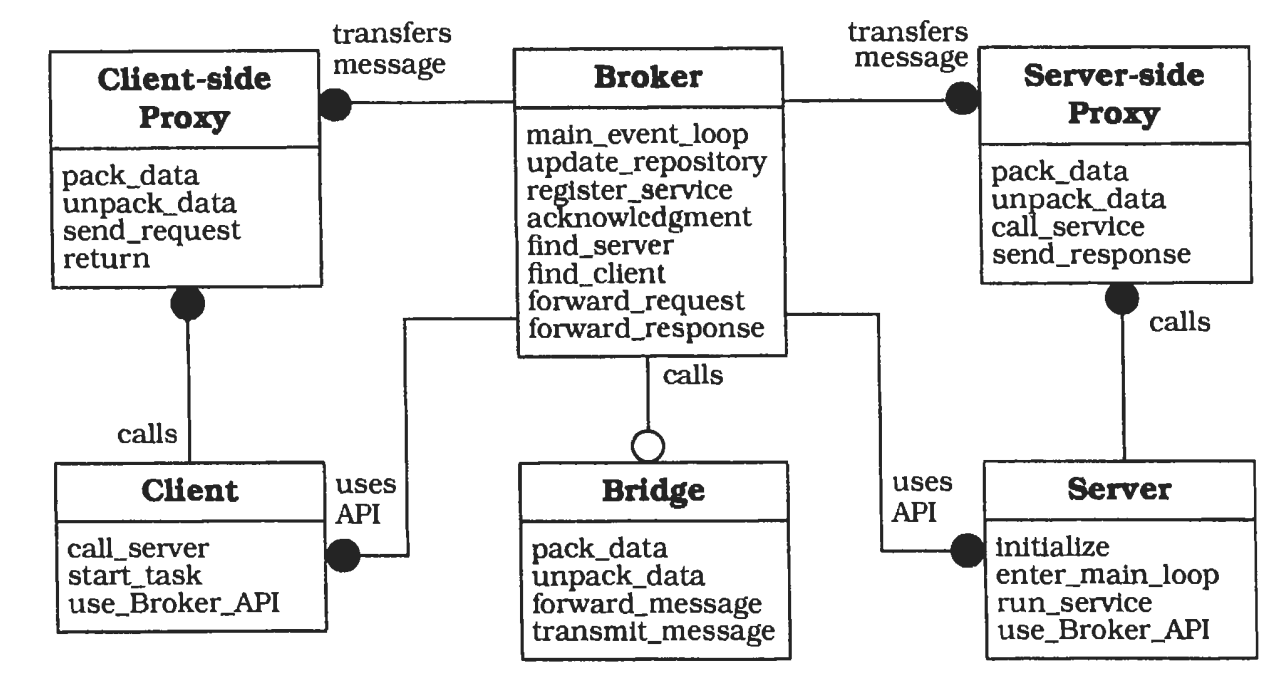
\includegraphics[width=0.8\textwidth]{figures/06-broker-1}
	\caption{Broker Struktur}
\end{figure}

\begin{figure}[H]
	\centering
	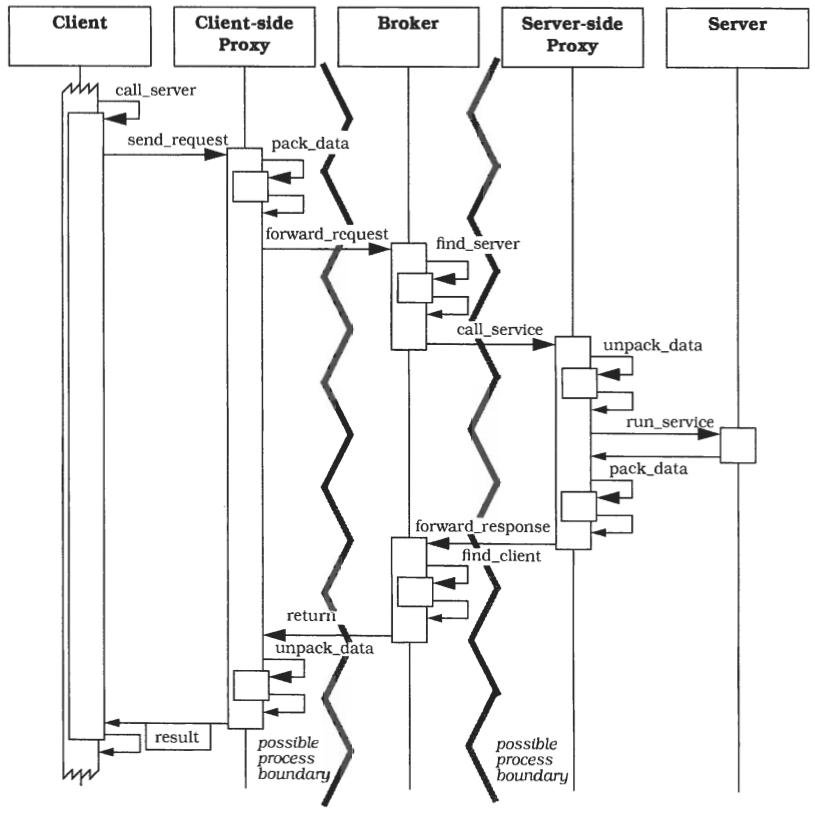
\includegraphics[width=0.8\textwidth]{figures/06-broker-2}
	\caption{Broker Sequenzdiagramm}
\end{figure}

\section{Variants}

\paragraph{Direct Communication Broker System}
In dieser Variante können Clients direkt mit dem Server kommunizieren. Der Broker teilt dem Client mit über welchen Kommunikationskanal der Server erreichbar ist.

\paragraph{Message Passing Broker System}
In dieser Variante stellen die Server keine Services zur Verfügung, sondern empfangen Messages und entscheiden anhand von deren Typ, was damit zu tun ist. Eine Message besteht dabei aus Rohdaten, sowie zusätzlichen Informationen welche den Typ, die Struktur und die Attribute der Message beschreiben.

\paragraph{Trader System}
Normalerweise wird ein Request zu einem einzigen eindeutig identifizierbaren Server weitergeleitet. In einem Trader System sind allerdings die Services und nicht die Server eindeutig identifizierbar. Ein Request kann somit an mehrere Server weitergeleitet werden, welche den gleichen Service implementieren.

\paragraph{Adapter Broker System}
In dieser Variante wird das Interface des Brokers gegenüber den Servern durch einen zusätzlichen Layer versteckt. Dadurch kann die Flexibilität erhöht werden. Der Adapter-Layer ist ein Teil des Brokers und ist verantwortlich für das Registrieren der Server und die Interaktion mit den Servern. Wenn mehr als ein Adapter angeboten wird, können damit verschiedene Strategien zur Granularität und dem Ort der Server unterstützt werden.

\paragraph{Callback Broker System}
Beim Ballback Broker System wird ein reaktives Kommunikationsmodell verwendet. Es wird dabei nicht zwischen Client und Server unterschieden. Wenn ein Event ankommt ruft der Broker die Callback-Methode derjenigen Komponente auf, welche registriert wurde auf den Event zu reagieren. Dieser Aufruf kann neue Events erzeugen welche wiederum den Broker dazu bringen können, weitere Callback-Methoden aufzurufen.

\section{Consequences}
\begin{itemize}
	\pro{Location Transparency}
	\pro{Changeability and extensibility of components}
	\pro{Portability of a Broker system}
	\pro{Interoperability between different Broker systems}
	\pro{Reusability}	
	\con{Restricted efficiency}
	\con{Lower fault tolerance}
\end{itemize}


\section{Known Uses}
\begin{itemize}
	\item CORBA
	\item IBM SOM/DSOM
	\item World Wide Web
	\item ATM-P
\end{itemize}

\section{Relationships}
\begin{itemize}
	\item \textit{Forwarder-Receiver Pattern}
	\item \textit{Proxy Pattern} 
	\item \textit{Client-Dispatcher-Server Pattern}
	\item \textit{Mediator design Pattern} 
\end{itemize}

\section{Exam Questions}
\begin{itemize}
	\item Behauptung: dies ist eine Behauptung? (Lösung)
    \item Frage: Dies ist eine Frage? (Lösung)
\end{itemize}
